% Block Diagram Example: PID Control System with Feedback
% Compile with: pdflatex block-diagram.tex
\documentclass[tikz,border=2mm]{standalone}

\usetikzlibrary{arrows.meta,positioning,calc}

% Grayscale palette
\definecolor{figdark}{gray}{0.25}
\definecolor{figlight}{gray}{0.85}

% Style definitions
\tikzset{
  block/.style={
    rectangle, draw=figdark, fill=figlight,
    minimum width=2cm, minimum height=0.8cm,
    text centered, font=\small\sffamily
  },
  terminal/.style={
    rectangle, draw=figdark, fill=white,
    minimum width=1.2cm, minimum height=0.6cm,
    text centered, font=\small\sffamily
  },
  sum/.style={
    circle, draw=figdark, fill=white,
    minimum size=5mm, inner sep=0pt,
    font=\scriptsize\sffamily
  },
  arrow/.style={->, >=Stealth, thick, draw=figdark}
}

\begin{document}
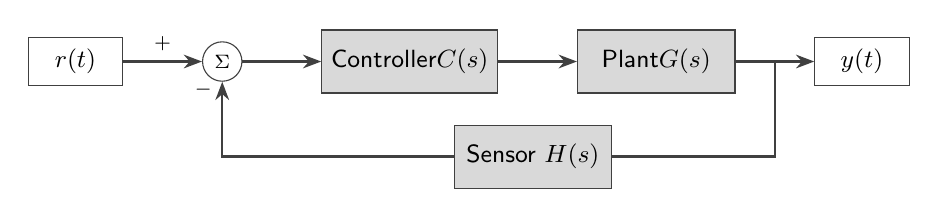
\begin{tikzpicture}[node distance=1cm]

  % Main signal path
  \node[terminal] (ref) {$r(t)$};
  \node[sum, right=of ref] (sum) {$\Sigma$};
  \node[block, right=of sum] (ctrl) {Controller\\$C(s)$};
  \node[block, right=of ctrl] (plant) {Plant\\$G(s)$};
  \node[terminal, right=of plant] (out) {$y(t)$};

  % Feedback path
  \node[block, below=0.8cm of $(ctrl)!0.5!(plant)$] (sensor) {Sensor $H(s)$};

  % Forward path connections
  \draw[arrow] (ref) -- node[above, font=\scriptsize] {$+$} (sum);
  \draw[arrow] (sum) -- (ctrl);
  \draw[arrow] (ctrl) -- (plant);
  \draw[arrow] (plant) -- (out);

  % Feedback loop
  \coordinate (fb) at ($(plant.east)!0.5!(out.west)$);
  \draw[thick, draw=figdark] (fb) |- (sensor.east);
  \draw[arrow] (sensor.west) -| (sum.south)
    node[pos=0.95, left, font=\scriptsize] {$-$};

\end{tikzpicture}
\end{document}
